% Unified working manuscript; no submission or editorial decision is implied.
% Existing frozen manuscripts, methods, and result fragments remain unchanged.
\documentclass[sigconf,nonacm]{acmart}
\usepackage{pvldb}
\renewcommand\vldbdoi{XX.XX/XXX.XX}
\renewcommand\vldbpages{XXX-XXX}
\renewcommand\vldbavailabilityurl{https://github.com/mandu5/sparse-vus/tree/research/saturation-20261021}
\newtheorem{theorem}{Theorem}
\newtheorem{lemma}{Lemma}
\newtheorem{proposition}{Proposition}
\newtheorem{corollary}{Corollary}
\newcommand{\ind}{\mathbf{1}}
\newcommand{\TP}{\mathrm{TP}}
\newcommand{\TPR}{\mathrm{TPR}}
\newcommand{\FPR}{\mathrm{FPR}}
\emergencystretch=2em
\begin{document}
\title{Sparse Events and Complete-Tie Prefixes for Exact VUS Evaluation}
\author{Youngmin Ko}
\email{rhdudals0505@naver.com}
\affiliation{\institution{Independent Researcher}\country{Republic of Korea}}
\begin{abstract}
Volume Under the Surface (VUS) evaluates anomaly scores across thresholds
and temporal tolerance widths. We derive an exact scalar event representation
for a pinned dynamic VUS definition: thresholds without active support have
analytically integrable contributions, while retained events preserve complete
global score ties. With standard binary64 radix ranking and interval geometry,
the evaluator takes $O(n+(L+1)Q)$ time, where $Q$ is maximum-buffer support.
Reversible activation and incremental component unions further reduce this to
$O(n+L+\alpha(K)\sum_wJ_w)$, where $J_w$ counts the active prefix through
recall saturation. For one original interval, spatial runs aggregate complete
score classes; an integer stopping certificate gives a run-sensitive bound
without restricting tie cardinality. A fixed-point range-sum implementation
has a local mass-error bound, distinct from exact real-arithmetic evaluation.
A frozen three-score-vector workload covers 308 series in 17 families and
924 series--width tasks per CPU platform. At primary width 30, sparse radix
passes its five-control criterion; median ratios against released fast-VUS
are $20.925\times$ and $14.538\times$, and against matched dense radix
$2.599\times$ and $4.791\times$. A separate incremental study finds that
saturation fails its default-width runtime criterion in all three runs,
with qualified gains at larger widths. Exactness concerns the exhaustive
mathematical target. Run aggregation helps structured large ties but does not
broadly improve the measured real-score runtimes. Numerical parity and
practical speed are separate claims. In a directly timed 308-file evaluation,
selection and output workflow, released sparse radix takes 3.187 seconds at the median, versus
11.298 seconds for matched dense radix and 63.647 seconds for fast-VUS,
with identical selected-model sets across all nine passes.
\end{abstract}
\maketitle
\vldbtopmatter
\section{Introduction}
Accuracy evaluation can itself be a repeated computational operation in
time-series anomaly studies. Volume Under the Surface (VUS) averages
range-aware ROC or precision--recall integrals across temporal tolerance
widths~\cite{paparrizos2022,boniol2025}. We study the evaluator after scores
have been produced: given labels, scores and a maximum width, compute the
same scalar for every distinct threshold and every integer width. Detector
training, score generation, data ingestion and downstream scientific choice
of the metric are outside this computational problem.

Existing acceleration already exploits substantial structure. Boniol
et al.'s Algorithms~2 and~3 partition maximum-buffer support from unaffected
regions and reuse static work~\cite{boniol2025}. Klein's fast-VUS sorts
support scores and computes weighted cumulative sums~\cite{klein2026}.
Benchopt supplies a dense cumulative-sum implementation~\cite{benchopt2026}.
The remaining question is which threshold states and width-dependent
preparations can be omitted while preserving the complete scalar integral.

Sparse VUS answers this question in stages. First, a score group with no
position in maximum support changes neither weighted positive mass nor
component coverage. It contributes zero PR area, but its ROC contribution
must be integrated before the next retained event. Complete global tie
counts preserve predictions outside support. Second, a two-distance
interval lemma and standard fixed-width ranking give an exhaustive
$O(n+(L+1)Q)$ evaluator for support size $Q$. Third, activating only current
support in score order avoids a full-support scan at each width; processing
ends when both mass and component coverage permanently saturate recall.
Finally, for one original interval, complete score classes can be aggregated
through their contiguous temporal runs. An integer sufficient condition
makes this stopping decision independent of rounded mass calculations.

These reductions account for features that distinguish the pinned target
from ordinary binary AUC: positive and negative denominators depend on
predicted buffer mass; expanded anomaly components merge with width; and
global score ties may combine active and inactive positions. The statements
are exact-arithmetic identities and operation-count bounds. Compiled
floating-point realizations and their numerical contracts are evaluated
separately; no bitwise identity or universal runtime advantage is inferred
from a theorem.

A preliminary support-event implementation and working manuscript were
publicly released as Sparse VUS~0.3.0 on 21 October
2026~\cite{sparsevus03}. This paper presents that evaluator together with
its prefix and complete-tie extensions. The public precursor is an
unsubmitted research artifact, not an earlier refereed publication. We
retain its versioned evidence and distinguish whole-evaluator improvements
from incremental improvements over that precursor.

The empirical distinction matters. A frozen 308-series study evaluates
three score vectors in each of 924 series--width tasks per platform;
the exact radix evaluator passes its primary five-control criterion on
both CPUs. A separate study measures individual score-vector calls and
finds that the active-prefix extension fails its default-width primary
criterion in all three runs. Larger-width improvements and slower cases
are reported together. The complete-tie extension is a separate candidate
with its own evidence; historical timings are not assigned to new code.

\section{Target and exact event representation}
Let $y\in\{0,1\}^n$ contain both classes and $s\in\mathbb{R}^n$ contain finite
scores after binary64 conversion. Larger scores indicate greater anomaly
evidence. Let $P_0=\sum_i y_i$, and let the $K$ maximal original anomaly
intervals have inclusive endpoints $[a_k,b_k]$ in temporal order. Widths are
the integers $w=0,\ldots,L$. The continuous label $a_i^{(w)}$ is one on
original positives. An interval contributes $\sqrt{1-d/w}$ outside its
endpoints at integer distance $1\le d\le\lfloor w/2\rfloor$; contributions
are summed and clipped at one. At $w=0$ no ramp is added. Expanded intervals
that overlap merge, while adjacent nonoverlapping intervals remain separate.
This is the original dynamic VUS target pinned to the official
\texttt{RangeAUC\_volume\_opt} source at revision
\texttt{467bace0}, configured for exhaustive thresholds~\cite{vusreference}.
It is not shared by all software named VUS.

For a threshold $t$, define
\begin{align}
 p_i(t)&=\ind\{s_i\ge t\}, & C(t)&=\sum_i p_i(t),\\
 A(t)&=\sum_i y_i p_i(t), &
 B(t)&=\sum_i(1-y_i)a_i^{(w)}p_i(t),\\
 T(t)&=A(t)+B(t), & P(t)&=P_0+B(t)/2,\\
 N(t)&=n-P(t).
\end{align}
Let $H(t)$ count expanded components hit by at least one predicted positive,
and let $K_w$ count those components. The curve coordinates are
\begin{align}
 R(t)&=\min\{T(t)/P(t),1\}\,H(t)/K_w,\\
 F(t)&=(C(t)-T(t))/N(t), & \pi(t)&=T(t)/C(t).
\end{align}
Precision is used only at nonempty retained thresholds, where $C(t)>0$;
the initial origin requires no precision value.
The denominator is positive: $P(t)\le(n+P_0)/2<n$. ROC integrates trapezoids
from the origin through complete distinct descending score thresholds to
the explicit terminal $(1,1)$. PR uses the right-step sum
$\sum_j(R_j-R_{j-1})\pi_j$, with $R_0=0$. Each VUS scalar is the arithmetic
mean over every width. Signed horizontal ROC increments are preserved; the
derivation does not replace a dynamic denominator by a fixed one.

Let $S_w=\{i:a_i^{(w)}>0\}$, $Q_w=|S_w|$, and $Q=Q_L$. For an active event
with score $v_j$, precompute the complete global counts
$c_j^>=|\{i:s_i>v_j\}|$ and $c_j^\ge=|\{i:s_i\ge v_j\}|$. They include
positions outside $S_w$ and outside $S_L$.

\begin{lemma}[Inactive threshold runs]
Between consecutive active score events at a fixed width, $T,B,P,N,H,R$
are constant. Omitted thresholds contribute a horizontal ROC rectangle and
zero PR area. At an active score, its complete global numerical tie is a
single transition.
\end{lemma}
\begin{proof}
A newly admitted inactive point has zero weight and cannot hit an expanded
component. Only $C$ changes. The horizontal increments
$(\Delta C)/N$ telescope at fixed height $R$. All positions tied with an
active event enter at its global threshold, so both counts must retain them.
\end{proof}

If the previous retained state is $(T_o,N_o,R_o,c_o)$, event $j$ contributes
\begin{align}
 f_j^-&=(c_j^>-T_o)/N_o,\\
 \Delta\mathrm{ROC}_j&=
 (c_j^>-c_o)R_o/N_o+(F_j-f_j^-)(R_j+R_o)/2,\\
 \Delta\mathrm{PR}_j&=(R_j-R_o)T_j/c_j^\ge.
\end{align}
The initial state is $(0,n-P_0,0,0)$, and afterwards $c_o=c_j^\ge$.
Connecting retained endpoints without the intervening rectangle is
incorrect. For example, $y=(1,0,1,0)$, $s=(3,2,1,0)$ and $L=0$ give ROC
area $0.625$; connecting support endpoints alone gives $0.8125$.

\begin{lemma}[Two-distance geometry]
The weight of a non-original point is determined by its distances $d_1,d_2$
to the nearest two distinct original intervals. It is zero if
$d_1>\lfloor w/2\rfloor$, one if $d_2\le\lfloor w/2\rfloor$, and
$\sqrt{1-d_1/w}$ otherwise.
\end{lemma}
\begin{proof}
Every active ramp has weight at least $1/\sqrt2$. Two contributions therefore
clip to one. If exactly one interval contributes, its distance determines
the weight. Distances to ordered intervals are monotone moving away on each
side, so two neighbors on each side contain the nearest two intervals.
\end{proof}

\begin{theorem}[Support-event evaluation]
\label{thm:support-events}
In a unit-cost model with score comparisons and metric arithmetic, including
square roots, both exhaustive scalar integrals can be computed in
$O(n\log(Q+1)+(L+1)Q)$ time and $O(n+Q)$ auxiliary words.
\end{theorem}
\begin{proof}
Extract original intervals and maximum support in $O(n)$ time. Sort the $Q$
support scores and group equal values. Binary-search all $n$ scores among
these groups to obtain complete global counts $c^>,c^\ge$ without sorting
off-support scores, at cost $O(n\log(Q+1))$. The ordered-interval geometry
can be prepared within this bound. At each width, compute support weights,
component membership, grouped masses and first component-hit events in
$O(Q+K)$ time. A scan of the at most $Q$ event groups integrates the
preceding rectangles, complete tied transitions and terminal ROC tail.
The inactive-run lemma makes this identical to the exhaustive target in
exact metric arithmetic. Stream the width mean using input-, support- and
interval-sized arrays. Since $K\le Q\le n$, the stated bounds follow.
\end{proof}

\begin{proposition}[Fixed-binary64 preparation]
\label{prop:radix}
For finite binary64 scores, complete global tie counts, the score ordering
of maximum support, and its two-distance geometry can be prepared in
$O(n+Q+K)$ time and $O(n+Q)$ auxiliary words. Discrete work uses a word-RAM
with input indices, counts, widths, and intermediate index arithmetic
fitting words. Metric arithmetic, including square roots, has unit cost.
\end{proposition}
\begin{proof}
Normalize signed zeros. Complement a negative score's bit pattern and flip
the sign bit of a nonnegative score, then complement the result to obtain a
descending numerical key. Eight stable byte-counting passes order these
64-bit keys in $O(n)$ time. Scan complete ties and retain their starting and
ending global ranks. Filter the permutation to maximum-support positions.
A temporal scan with a monotone interval pointer computes nearest distances
and owners in $O(Q+K)$ time. All arrays are input- or support-sized.
\end{proof}
Radix sorting and floating-point key transforms are established
techniques~\cite{demaine2011radix,herf2001radix}. This assumption does not give
linear sorting of arbitrary real scores or a bit-complexity bound for growing
precision. Conversion defines numerical ties, including collisions between
distinct large integer inputs.

The same support-event width kernel combined with this preparation gives
$O(n+(L+1)Q)$ time. This is the basic Sparse VUS evaluator; its improvement
over a dense rank sweep depends on $Q$, rather than recall saturation.
The released PR-only implementation retains $L+1$ scalar width results,
adding $O(L)$ words; streaming removes this storage. Input-sized ranking
arrays remain necessary in this construction, so the memory is not
support-only.

\section{Prior algorithms and comparison scope}
Boniol et al.'s optimized VUS algorithms retain threshold loops within
widths and support-region summation~\cite{boniol2025}. The official source
additionally creates full-length prediction and label arrays per threshold.
Klein removes repeated threshold-wise summation through support cumsums,
but still constructs maximum-support and full-length coverage arrays at
each width~\cite{klein2026}. Benchopt cumsums over all positions and computes
component-hit counts through segment maxima~\cite{benchopt2026}.
Table~\ref{tab:algorithm-scope} distinguishes these mechanisms from the
new reductions. Its costs describe inspected operations, not cross-library
runtime predictions.

\begin{table*}[t]
\centering\small
\setlength{\tabcolsep}{4pt}
\begin{tabular}{p{0.19\textwidth}p{0.29\textwidth}p{0.43\textwidth}}
\toprule
Construction & Threshold and width work & Semantic/comparison qualification\\
\midrule
Boniol Algorithms 2/3 & Per-width threshold loop; $Q$-support sums per threshold & Static-support reuse and cached predictions are prior techniques; the released target uses $\ge$ ties.\\
Klein fast-VUS & Per-width support cumsum, full-series coverage and threshold arrays & PR only; use $H=n$, not the sampled default $H=250$. Explicit arrays cost $\Omega(Q+n+H)$ per width.\\
Benchopt & Per-width full-series cumsum and threshold arrays & Computes both ROC and PR; $H=n$ covers exhaustive ties. Explicit arrays cost $\Omega(n+H)$ per width.\\
FF-VUS & Batched width/threshold matrices and support masking & Native linear/max ramps differ from the pinned target; public wrapper rounds scores; Torch has an existence approximation fallback.\\
Sparse support events & $O(n+(L+1)Q)$ with fixed-key preparation & Removes inactive thresholds while retaining global counts and exact ROC rectangles; no prefix stop is required.\\
Active positions & $O(n+L+\alpha(K)\sum_wJ_w)$ & Complete terminating active ties; arbitrary components; worst-case $J_w=Q_w$.\\
Complete-tie runs & $O(n+L+\sum_w\sum_{g\in\mathcal G_w}R_g)$ & One original interval; charges all stored runs of every visited class; integer stopping certificate.\\
\bottomrule
\end{tabular}
\caption{Algorithmic comparison. $H$ is the requested threshold count;
$Q$ is maximum support; $J_w$ counts visited active positions; $R_g$ counts
temporal runs of score class $g$. External array-cost lower bounds omit
additional ramp, sorting and search work. Batched FF-VUS has no single
sequential per-width loop. Our bounds use the stated arithmetic model.}
\label{tab:algorithm-scope}
\end{table*}

Sorted sweeps, complete ties and trapezoids are established ROC
techniques~\cite{fawcett2006}. scikit-learn~1.0.2 explicitly truncates PR at
full recall after forming cumulative counts~\cite{sklearn102}. Therefore
full-recall stopping and zero-area PR suffixes are not new principles.
Our comparison includes last-original-positive stopping, which already
ensures saturation. The specific questions are whether buffer mass permits
an earlier stop and whether preparation avoids paying for the discarded
suffix. Reversible list updates~\cite{knuth2000}, union-find~\cite{tarjan1984},
radix ordering~\cite{demaine2011radix,herf2001radix} and exact
accumulators~\cite{neal2015} are established tools used in the construction.

Sylligardos reports preliminary CPU/GPU VUS acceleration~\cite{sylligardos2025}.
The public FF-VUS code attributed to him in aVUSi~\cite{ffvus2026} uses a
different ramp/overlap contract; its wrapper rounds scores, and Torch can
interpolate component existence across widths when memory is insufficient.
This is relevant acceleration prior art, but its native runtime is not an
exact-target comparison. No result here establishes superiority over an
unmeasured GPU evaluator. Source pins and minimal semantic witnesses are
retained with the artifact; a package name alone does not establish equality.

\section{Prefix evaluation without full-support setup}
\begin{figure}[t]
\begin{minipage}{\linewidth}
\textbf{Once:} rank complete global ties; prepare interval distances and
owners; schedule activations/unions; record reverse-deletion neighbors.\\[2pt]
\textbf{For each width:} restore newly active positions and merge overlapping
intervals; start mass, hit count and areas at zero.\\[2pt]
\textbf{For each complete active score tie:} update weighted mass and component
hits; integrate its preceding negative rectangle and tied transition.\\[2pt]
\textbf{Stop:} if $A+B/2\ge P_0$ and $H=K_w$, append ROC tail $1-F$;
the remaining PR area is zero. Stream the width means.
\end{minipage}
\caption{Position-prefix evaluator. No width clears or scans a support-sized
or component-sized array before traversal.}
\Description{An offline schedule maintains current support in score order and
components across widths, then scans complete ties to permanent saturation.}
\label{fig:sparse-prefix}
\end{figure}
\subsection{Exact evaluation of active score prefixes}
\label{sec:saturation}
At a fixed width, let $A$ count admitted original-positive positions and let
$B$ denote their admitted non-original buffer mass. Then $T=A+B$ and
$P=P_0+B/2$. We call a complete score threshold \emph{saturated} when
\begin{equation}
 A+B/2\ge P_0\qquad\hbox{and}\qquad H=K_w.
 \label{eq:saturation-condition}
\end{equation}
The condition includes the complete global numerical tie, even when only some
positions in that tie belong to the width's active support.

\begin{lemma}[Permanent saturation]
After a threshold satisfying~\eqref{eq:saturation-condition}, every subsequent
recall coordinate equals one. The remaining right-step PR contribution is
zero, and the remaining trapezoidal ROC contribution, including the explicit
terminal $(1,1)$ transition, is $1-F$, where $F$ is the current FPR.
\end{lemma}
\begin{proof}
Threshold relaxation cannot decrease $A$, $B$, or the number of hit expanded
components. Thus both conditions persist. The first is equivalent to
$(A+B)/(P_0+B/2)\ge1$; the second makes the existence factor one. Every later
PR recall increment vanishes. Every later ROC trapezoid has height one, so
its signed horizontal increments telescope from the current $F$ to the
terminal abscissa one. The proof does not assume a fixed negative denominator.
\end{proof}

Stopping at recall one is a standard flat-curve observation, not a claimed
new integration principle. In particular, admitting the last original
positive gives $A=P_0$ and hits every expanded component, so it is already a
valid cutoff. The VUS-specific condition can stop earlier: buffer mass can
compensate for original positives that have not yet been admitted. Both
last-original-positive stopping and disabled stopping are explicit controls.

A cutoff added after constructing every width's full support histogram would
still pay $\Theta(Q)$ per width. To avoid that work, retain support positions
in descending score order, and activate position $i$ at radius $d_1(i)$;
original positives have activation radius zero. The score-ordered list is
represented by integer next pointers. Bucket-sort activations by their
integer radius. Starting from the full list, delete positions in reverse
activation order and record the two neighbors at each deletion. Reversing
these deletions inserts every position in constant time. Tied activation
radii use the same fixed order in both directions. Consequently traversing
the current list visits only positions with nonzero weight at that width.
A complete retained event still uses its precomputed global $c^>,c^\ge$;
points omitted from the current list may belong to that same global tie.

For geometry, preprocessing also records one nearest original interval for
each support position. At radius $r$, neighboring original intervals with
endpoints $b_k,a_{k+1}$ merge precisely when
$2r\ge a_{k+1}-b_k$. Bucket these edges by
$\lceil(a_{k+1}-b_k)/2\rceil$ and maintain their components with union-find.
Mere adjacency of expanded intervals does not merge them. An active point
lies in its nearest interval's expansion. Any other expansion containing the
point overlaps that expansion and belongs to the same component; hence the
nearest interval's union-find root identifies the point's component. A
width-stamped root array counts first hits without clearing all components
at each width. Unions occur before a width's threshold scan, so roots are
fixed throughout that scan.

\begin{theorem}[Active-prefix bound]
Use the fixed-binary64 word-RAM and unit-cost metric-arithmetic assumptions
of Proposition~\ref{prop:radix}. Let $J_w$ be the number of active support
positions visited through the complete first saturated score tie at width
$w$, and let $K$ count original intervals. Both scalar integrals can be
computed in
\[
 O\!\left(n+L+\alpha(K)\sum_{w=0}^{L}J_w\right)
\]
time and $O(n+Q)$ auxiliary words, where $\alpha$ denotes the inverse
Ackermann factor for union-find. A diagnostic vector of per-width work
counts uses an additional $O(L)$ words. The values equal the target
integrals in exact metric arithmetic.
\end{theorem}
\begin{proof}
Fixed-width radix ranking, complete global tie counts, the nearest-interval
scan, and extraction of the ordered support take $O(n+Q+K)$ time.
All activation distances and finite merge radii are at most $n-1$, so
bucket arrays are capped at $\min(\lfloor L/2\rfloor,n-1)+1$, even if $L$
is much larger than $n$. Counting-sort schedules and reverse deletions take
$O(n+Q+K)$ time and space. Each position is activated once, and there are
at most $K-1$ unions. Union by size with path compression takes amortized
$O(\alpha(K))$ per operation. Every visited position performs one find;
event arithmetic and first-hit accounting take constant additional time.
No width requires an additional $Q$- or $K$-sized scan. Streaming the means
requires $L+1$ width iterations. Since at width zero saturation requires all
original positives, $J_0=P_0\ge K$, and the union cost is absorbed by
$\alpha(K)\sum_w J_w$. Active-event elimination uses the same negative-run
rectangles as before, and the lemma supplies the exact omitted suffix.
All scratch state is input-, support-, or interval-sized.
\end{proof}

The bound is adaptive, not a worst-case improvement for every score vector:
$J_w$ may equal the full active support size. Union-find and linked-list
access also have costs that a work-count reduction does not measure.
Nevertheless, a separating family exists even against the same active-list
algorithm stopped at the last original positive. For $L\ge2$, take
$n=4L+3$, with singleton originals at zero-based positions $L+1$ and $3L+1$.
Rank first the first original, then its two immediate neighbors, then one
immediate neighbor of the second original. Rank the second original last;
put all remaining scores strictly between the fourth and last scores.
At every width $w\ge2$, those three neighbors have weight at least
$1/\sqrt2$, so the first four active positions satisfy
\[
 A+B/2\ge 1+\frac{3}{2\sqrt2}>2=P_0
\]
and hit both expanded components. Thus $J_w=4$, while at widths zero and
one $J_w=2$. The last-original-positive control must traverse
$Q_w=4\lfloor w/2\rfloor+2$ active positions at every width, giving
$\Theta(L^2)$ traversal rather than $\Theta(L)$. With $K=2$ and $n=\Theta(L)$,
the full adaptive algorithm takes $O(n+L)$ on this family. This is a
structural operation-count separation, not an empirical runtime claim.

The implementation uses finite-precision arithmetic and can differ from a
full scan through summation order and suffix telescoping. The theorem is an
exact-arithmetic identity; measured numerical parity, floating-point limits,
and runtime comparisons must be reported separately.


\subsection{A uniform one-interval guarantee}
Every active original contributes one to $A+B/2$. Every active non-original
contributes at least $1/(2\sqrt2)$, because its half-width ramp is at least
$1/\sqrt2$. After any $q$ admitted active positions, mass is therefore at
least $q/(2\sqrt2)$, even inside a tie. Only complete ties are admissible
thresholds.
\begin{proposition}[Distinct active scores in one interval]
If $K=1$ and scores in $S_L$ are pairwise distinct after binary64 conversion,
then $J_w\le\min\{Q_w,\lceil2\sqrt2 P_0\rceil\}$ for every width and score
ordering. The position-prefix evaluator takes $O(n+LP_0)$ time. A singleton
has $J_w\le3$ and $O(n+L)$ time.
\end{proposition}
\begin{proof}
The first active position hits the only expanded component. The preceding
mass inequality ensures saturation by $\lceil2\sqrt2P_0\rceil$ positions;
if support is smaller, admitting it all includes every original and
saturates. Distinct active scores permit stopping after each position.
Union-find is constant work for one interval, and summing over widths gives
the bound; $P_0\le n$ absorbs the additional width-zero term.
\end{proof}

The guarantee needs no score-quality assumption. It does require distinct
\emph{active} scores: exclusively off-support ties do not enlarge active
events. For an all-tied singleton, a complete event contains $Q_w$ active
positions and the position-wise evaluator can perform $\Theta(L^2)$ total
visits when $n=\Theta(L)$. This is a limitation of that evaluator, not a
problem lower bound. For multiple components, a low-scoring component can
also force a long coverage prefix after enough mass has accumulated.
The next construction addresses tied-position enumeration for one interval.

\subsection{Complete-tie aggregation for one original interval}
\label{sec:tie-run-method}
This subsection describes a separate candidate evaluator. It does not alter
the frozen position-by-position evaluator or its recorded measurements.
Assume there is exactly one original interval $[a,b]$, with
$P_0=b-a+1$. Its maximum support $S_L$ is a single interval. For each
validated numerical score class $g$ in $S_L$, store its maximal contiguous
spatial runs, and let $R_g$ be their number. These runs are defined in the
maximum support, not separately at each width. A class becomes active when
the width radius first reaches the minimum distance of one of its positions
from $[a,b]$. Classes, rather than individual positions, can therefore use
the same reverse-deletion insertion schedule, in descending score order.
Global prediction counts still include every position in a complete global
tie, including positions outside $S_L$.

\begin{lemma}[A ramp run is one square-root range sum]
Let $w\ge2$, and let a nonempty run fragment on one side of $[a,b]$
have active distances $1\le d_-\le d_+\le\lfloor w/2\rfloor$.
Writing $U(t)=\sum_{j=1}^{t}\sqrt j$, with $U(0)=0$, its buffer mass is
\[
 \sum_{d=d_-}^{d_+}\sqrt{1-d/w}
 =\frac{U(w-d_-)-U(w-d_+-1)}{\sqrt w}.
\]
Every stored run has at most two such fragments and one original fragment.
Thus its exact mass and admitted-position counts require constant work
given exact range sums. At widths zero and one, only the original fragment
contributes.
\end{lemma}
\begin{proof}
The distance to a single interval changes by one at consecutive positions
on either side. The identity follows from
$\sqrt{1-d/w}=\sqrt{w-d}/\sqrt w$ and reversing the summation order.
Intersections with the left ramp, original interval, and right ramp
are interval intersections and require constant work.
\end{proof}

\begin{lemma}[Integer saturation certificate]
\label{lem:integer-saturation}
At the end of a complete active score class, let $A$ count admitted original
positions and let $D$ count admitted non-original active positions. The test
\[
 \left\lfloor D/3\right\rfloor\ge P_0-A
 \label{eq:integer-saturation}
\]
certifies true mass-and-coverage saturation. It uses only integer counts,
and the test $D\mathbin{//}3\ge P_0-A$ avoids multiplication overflow.
It may stop later than the real-valued mass test. Nevertheless, the
number of complete active score classes visited at any width is at most
$3P_0$, without any tie-size assumption.
\end{lemma}
\begin{proof}
Every active non-original weight is at least $1/\sqrt2>2/3$, hence
$B/2\ge D/(2\sqrt2)\ge D/3$. The certificate implies
$A+B/2\ge P_0$. There is one expanded component, hit by the first active
class. If $q=A+D\ge3P_0$ positions have been admitted, then
$D=q-A\ge3P_0-3A$, so the certificate holds. If fewer than $3P_0$
active positions exist, admitting them all gives $A=P_0$ and also
certifies saturation. Each visited active class contains at least one
new position. Consequently, after at most $3P_0$ complete classes the
certificate holds, regardless of the cardinality of those classes.
\end{proof}

Let $\mathcal G_w$ be the classes visited through the first complete
class satisfying the integer certificate. The bound below charges all
$R_g$ maximum-support runs of each visited class, including those inactive
at that particular width.

\begin{theorem}[Tie-run work bound]
\label{thm:tie-run-bound}
Under the fixed-key and unit-cost exact metric-arithmetic model, the ideal
run-aggregated evaluator computes both scalar integrals in
\[
 O\!\left(n+L+\sum_{w=0}^{L}\sum_{g\in\mathcal G_w}R_g\right)
\]
time and $O(n+L)$ auxiliary words. For
$R_{\max}=\max_g R_g$, its time is
$O(n+L+(L+1)P_0R_{\max})$.
For a singleton original and bounded $R_{\max}$, it is $O(n+L)$ even
with arbitrary active tie cardinalities. If all support scores are tied,
it is $O(n+L)$ for every one-interval length $P_0$.
\end{theorem}
\begin{proof}
Radix ranking, global tie counts, temporal run extraction, class activation
distances, and the offline class insertion schedule take $O(n)$ time and
space. Each class is inserted once. The $L+1$ square-root prefixes take
$O(L)$ time and space in exact metric arithmetic. A visited class costs
$O(R_g)$ to compute its mass and counts. The one-component existence factor
requires constant work. After the complete class, the standard
negative-run rectangle, event trapezoid, and right-step PR formulas use
these exact event aggregates. Lemma~\ref{lem:integer-saturation} makes the
omitted suffix valid by permanent saturation. Summing gives the first
bound; $|\mathcal G_w|\le3P_0$ gives the second. For an all-tied support,
there is one class containing one run, visited once per width.
\end{proof}

The hypothesis is on score-class fragmentation, not the number of distinct
scores. An alternating high/low score pattern can give $R_g=\Theta(n)$,
so this theorem is not a universal linear-time result for arbitrary ties.
The extra $O(L)$ prefix storage is present even without diagnostics. It
differs from the frozen evaluator's $O(n+Q)$ auxiliary-space bound.

\paragraph{A cancellation-free finite-precision range-sum implementation.}
Fixed-point superaccumulators are established summation techniques~\cite{neal2015}.
Subtracting two ordinary floating-point square-root prefixes can lose
relative accuracy on short ranges. Instead, let $q_j$ be the binary64
evaluation of $\sqrt j$ and accumulate the integers $2^{52}q_j$ exactly.
For $1\le j\le L\le2^{63}-1$, $1\le q_j<2^{32}$, and every
$2^{52}q_j$ is an integer below $2^{84}$. Every prefix is therefore below
$2^{147}$ and fits in three unsigned 64-bit limbs. Carry and borrow
operations give exact integer prefixes and exact range subtraction in a
constant number of word operations. If a nonnegative range difference
has limbs $(h,m,\ell)$, high to low, convert it by
\[
 \operatorname{fl}\!\left(
   2^{76}\operatorname{fl}(h)
   +2^{12}\operatorname{fl}(m)
   +2^{-52}\operatorname{fl}(\ell)\right),
\]
then divide by the evaluated $\sqrt w$. All additions are nonnegative;
there is no subtraction of rounded large prefixes. This preserves the
stated operation and storage bounds, up to a constant of three words per
prefix. It exactly sums the \emph{rounded} square-root table, not symbolic
square roots.

\begin{proposition}[Local range-mass error]
Assume binary64 round-to-nearest operations, the usual relative error
bound for integer conversion and square root, no reassociation, and exact
limb arithmetic. Put $u=2^{-53}$ and $\gamma_k=ku/(1-ku)$.
The preceding implementation's nonempty ramp-fragment mass $\widehat B$
satisfies
\[
 \left|\widehat B/B-1\right|\le\gamma_8.
\]
If every table index and width is at most $2^{53}$, $\gamma_6$ suffices.
These bounds do not grow with the prefix index or the fragment length.
Summing $t$ nonempty fragment masses using ordinary positive additions
gives a relative bound $\gamma_{t+7}$, provided $(t+7)u<1$.
\end{proposition}
\begin{proof}
Integer conversion followed by square root places each $q_j/\sqrt j$
between $(1-u)^2$ and $(1+u)^2$. Exact nonnegative summation preserves
these bounds. Conversion of each limb and two nonnegative additions add
at most three rounding factors; power-of-two scaling is exact and in
range. Division adds one factor, and the evaluated denominator contributes
at most two factors. Thus the final ratio lies between
$(1-u)^6/(1+u)^2$ and $(1+u)^6/(1-u)^2$, contained in
$[1-\gamma_8,1+\gamma_8]$. Exact integer conversion removes one factor
from both numerator and denominator, yielding $\gamma_6$. The standard
positive-sum product bound combines $\gamma_8$ with $\gamma_{t-1}$ to
give $\gamma_{t+7}$.
\end{proof}

This is a local mass-error bound. It is not an end-to-end error certificate
for the integrated scalar metrics, nor a claim of bitwise agreement with
the frozen $\sqrt{1-d/w}$ evaluation. The integer stopping certificate
is independent of these mass-rounding errors, but metric arithmetic and
summation still use finite precision. The work bound does not imply runtime
dominance; the experiments examine both compressible and fragmented ties.


\subsection{Implementation and arithmetic scope}
The support-event and position-prefix implementations expose both PR-only
and paired ROC--PR calls. Validation, score conversion and all preparation
belong to the public call. The PR route omits ROC arithmetic; diagnostics
that return per-width work counts are outside metric timing. Position-prefix
ablations use identical preparation but either disable stopping or stop at
the last original positive. The complete-tie candidate uses a separate
integer sufficient condition and its own measured scope.

All integer widths are evaluated. Consecutive widths with the same radius
can have different ramp weights: for $y=(0,1,0)$ and $s=(2,1,0)$, width-two
PR is approximately $0.77705$ and width-three PR approximately $0.85505$.
Reusing an area merely because $\lfloor w/2\rfloor$ is unchanged would alter
the target.

The position-prefix mass test uses floating point in the implementation;
its real-arithmetic proof is not a directed-rounding certificate. The
complete-tie integer certificate avoids that particular stopping uncertainty,
but its local range-mass bound is not an end-to-end integrated-scalar error
bound. Both implementations can differ from a full scan through rounded
roots, accumulation order and suffix telescoping. Numerical tolerances and
independent-reference checks are reported separately from the exact identities.

\section{Experimental design and evidence separation}
We distinguish two frozen studies with different task units and different
questions. Neither trains or queries a detector during evaluation timing.
The new complete-tie candidate has a separate evidence record; it does not
inherit either study's timings.

\paragraph{Whole-evaluator study.}
The v3 policy holdout uses 308 series from 17 represented families of the
previously studied corpus, with the released Chronos-Bolt base, Time-MoE
200M and TimesFM~1.0 200M score vectors at context length
64~\cite{zhu2026,tsbad}. It is a held-out policy evaluation within previously
studied source families, not a new-domain dataset. Each task is one
\emph{series--maximum-width} pair: evaluate all three frozen score vectors
and return the best-PR model set under the frozen numerical tie convention.
There are $308\times3=924$ tasks per platform for maximum widths 30, 100 and
300, with 308 primary tasks at width~30. This is distinct from 924 individual
score-vector calls. It measures metric evaluation and a fixed three-way
comparison, not end-to-end model selection or detector quality.

The exact sparse-radix evaluator is compared with five frozen controls:
comparison-based sparse PR, direct dense PR, nearest-distance dense ROC--PR,
direct dense radix PR, and nearest-distance dense radix PR. The matched
radix controls share fixed-key ranking, and the nearest control shares
interval geometry; their full-series width traversal isolates support-event
compression from those ingredients. Actual pinned Klein PR and Benchopt
ROC--PR are additional descriptive external comparisons, outside the
five-control decision. All use exhaustive thresholds and widths. Paired
outputs are explicitly marked in the tables.

Complete-task timings include validation and preparation for the three
score vectors. Three warmed repetitions run serially in seeded randomized
method order with one compute thread. Data I/O, imports and declared JIT
warmup are excluded. The primary decision requires numerical agreement and
lower 95\% family-cluster bootstrap bounds above one for both geometric and
aggregate ratios against every frozen control. The artifact retains the
exact inputs, sources, raw timings and decisions. The absolute numerical
parity tolerance is $10^{-11}$; selected-model ties use absolute tolerance
$10^{-10}$.
Apple M1 Pro and hosted Linux results are separate runs; software versions,
process snapshots and source hashes are recorded per run. They are not
pooled, and environment differences are not experimentally separated.

\paragraph{Incremental position-prefix study.}
Here a case is one \emph{series--score-vector--maximum-width} PR call. The
candidate is compared with eight controls: full active traversal,
last-positive stopping, released sparse radix, nearest dense radix,
Klein fast-VUS, comparison-based sparse, comparison-based direct dense,
and direct dense radix. All nine methods compute PR only. Klein receives
$n$ ranked thresholds; repeated ties have zero recall increments.

The development set has 42 previously studied series and three released
score vectors per series. The external set was selected from mTSBench
metadata before generating scores or observing metric outcomes~\cite{mtsbench}:
exclude the 23 earlier source-family names with recorded alias normalization,
restrict test lengths to 100,000, and take the lexicographically first two
eligible series per family. This yields 12 series from nine source families
and 457,171 rows. Source-family disjointness does not establish independent
real-world domains; synthetic and reused data are identified in the manifest.
Four fixed label-free CPU procedures generate score vectors: Isolation Forest,
standardized PCA reconstruction, reference-set nearest-neighbor distance,
and robust marginal deviation. These are evaluation inputs, not detector
leaderboard claims; their generation is outside timing.

Widths 30, 100 and 300 give 378 development cases and 144 external cases
per host. Each primary external width has 48 score vectors from 12 series.
Three randomized warmed serial repetitions include all public-call work;
imports, I/O, JIT warmup and diagnostic profiling are excluded. Libraries
and Numba use one compute thread. The primary criterion requires maximum
absolute PR discrepancy at most $10^{-11}$ and both 95\% family-cluster
bootstrap lower bounds above one against each of the eight controls at
width~30. Its 2,000 family resamples quantify observed family/case variation,
not three-repeat timing uncertainty or a population of all possible domains.
The Mac uses M1 Pro/Python~3.12.4; the hosted Ubuntu~24.04 runner reports
EPYC~9V74/Python~3.12.15. Both use NumPy~1.26.4 and Numba~0.59.1 for this
study. These versions are not assumed for the earlier whole-evaluator study.

For all reported ratios the numerator is control time and the denominator
is candidate time. The two preceding studies' aggregate ratios divide sums
of per-case median times; they are not directly timed application batches.
Section~\ref{sec:collection-workflow} separately times a complete stored-score
collection operation, including input reads and output serialization.
No primary decision is
replaced by a favorable secondary width or a post-measurement comparator.

\section{Results}
% Layout-only copy of frozen pr_engine_results.tex; all numbers/text unchanged.
\subsection{Frozen v3 policy holdout: exact radix evaluation}
\label{sec:pr-engine-results}
Each platform completed all 924 tasks on the same 308 series in 17 families,
with $L=30$ primary, $L=100$ secondary, and $L=300$ a stress regime.
Each task evaluates the three frozen model score vectors and returns the best-PR model set, retaining numerical ties.
Times include whole-task preparation and use the median of three repetitions.
The maximum absolute PR discrepancy from the comparison-sort sparse PR reference was
$1.554\times 10^{-15}$ on Mac and $1.332\times 10^{-15}$ on Linux.
These are numerical agreement checks for the pinned target.

The frozen exact-radix decision at $L=30$ is Mac: \textbf{PASS}; Linux: \textbf{PASS}.
It requires both the geometric-mean and aggregate-ratio lower confidence bounds
to exceed one against every one of the five frozen controls, together with correctness.
Klein and Benchopt comparisons are descriptive and are outside this decision.
Table~\ref{tab:radix-primary} retains every primary control and both external implementations.

All ratios are comparator time divided by exact sparse-radix PR time; values above one favor radix PR.
Brackets contain audited 95\% family-cluster bootstrap intervals (2000 resamples).
The aggregate ratio divides sums of per-case median times; it is not an observed batch wall time.
Intervals describe variation across families, not uncertainty in three timing repetitions.
F/S/T counts cases where radix PR is faster/slower/tied. Decisions use unrounded bounds.

\begin{table*}[t]
\centering\small
\setlength{\tabcolsep}{3pt}
\caption{Primary $L=30$: all 308 cases per platform. $\dagger$ marks the five frozen decision controls. R+P methods compute both ROC and PR; the others compute PR only. Dense direct and dense nearest use comparison sorting unless labelled radix.}
\label{tab:radix-primary}
\resizebox{\linewidth}{!}{%
\begin{tabular}{llrrrr}
\toprule
Platform & Comparator & Median & Geomean [CI] & Aggregate [CI] & F/S/T \\
\midrule
Mac & Sparse comparison$^{\dagger}$ & 1.774 & 1.620 [1.421, 1.920] & 1.960 [1.511, 2.323] & 271/37/0 \\
Mac & Dense direct$^{\dagger}$ & 3.331 & 3.160 [2.772, 3.506] & 4.255 [3.349, 5.112] & 306/2/0 \\
Mac & Dense nearest (R+P)$^{\dagger}$ & 5.050 & 4.840 [4.356, 5.368] & 6.140 [4.974, 7.181] & 308/0/0 \\
Mac & Dense direct radix$^{\dagger}$ & 2.677 & 2.617 [2.318, 2.870] & 3.595 [2.752, 4.514] & 303/5/0 \\
Mac & Dense nearest radix$^{\dagger}$ & 2.599 & 2.519 [2.297, 2.726] & 3.298 [2.624, 3.980] & 307/1/0 \\
Mac & Klein fast-VUS & 20.925 & 22.360 [19.764, 24.238] & 19.450 [17.910, 20.623] & 308/0/0 \\
Mac & Benchopt (R+P) & 35.420 & 37.572 [34.754, 41.101] & 37.990 [34.728, 42.965] & 308/0/0 \\
\midrule
Linux & Sparse comparison$^{\dagger}$ & 1.987 & 1.916 [1.839, 2.013] & 1.955 [1.745, 2.095] & 304/4/0 \\
Linux & Dense direct$^{\dagger}$ & 4.894 & 4.161 [3.170, 5.008] & 5.385 [4.241, 6.191] & 308/0/0 \\
Linux & Dense nearest (R+P)$^{\dagger}$ & 6.917 & 5.890 [4.639, 6.923] & 7.214 [5.688, 8.187] & 308/0/0 \\
Linux & Dense direct radix$^{\dagger}$ & 4.419 & 3.756 [2.904, 4.486] & 4.708 [3.794, 5.276] & 308/0/0 \\
Linux & Dense nearest radix$^{\dagger}$ & 4.791 & 4.047 [3.142, 4.821] & 5.010 [3.933, 5.643] & 306/2/0 \\
Linux & Klein fast-VUS & 14.538 & 13.814 [11.639, 15.930] & 11.232 [10.034, 12.514] & 308/0/0 \\
Linux & Benchopt (R+P) & 21.493 & 20.973 [18.481, 23.617] & 22.991 [19.193, 30.937] & 308/0/0 \\
\bottomrule
\end{tabular}}
\end{table*}

\paragraph{Secondary and stress regimes.}
Table~\ref{tab:radix-secondary} gives both matched PR-only radix dense controls at $L=100$ and $L=300$.
These controls share fixed-width score ordering with sparse radix and retain full dense width sweeps.
Their ratios assess the support-event reduction after matching the ranking implementation.
The full bound reports retain every other comparator, family effect, and slower case at each width.

\begin{table*}[t]
\centering\small
\setlength{\tabcolsep}{3pt}
\caption{Secondary and stress widths: all 308 cases per row, matched PR-only controls. Ratio direction and intervals follow Table~\ref{tab:radix-primary}.}
\label{tab:radix-secondary}
\resizebox{\linewidth}{!}{%
\begin{tabular}{lllrrrr}
\toprule
Platform & $L$ & Comparator & Median & Geomean [CI] & Aggregate [CI] & F/S/T \\
\midrule
Mac & 100 & Dense direct radix & 5.110 & 4.834 [3.728, 5.802] & 6.874 [4.488, 8.943] & 307/1/0 \\
Mac & 100 & Dense nearest radix & 4.637 & 4.551 [3.602, 5.370] & 6.096 [4.117, 7.577] & 305/3/0 \\
Mac & 300 & Dense direct radix & 6.916 & 6.534 [4.259, 8.903] & 8.850 [5.163, 12.681] & 308/0/0 \\
Mac & 300 & Dense nearest radix & 6.294 & 6.000 [3.902, 8.163] & 7.892 [4.670, 11.080] & 300/8/0 \\
Linux & 100 & Dense direct radix & 7.465 & 6.666 [4.438, 8.952] & 8.220 [5.435, 10.714] & 308/0/0 \\
Linux & 100 & Dense nearest radix & 7.919 & 6.975 [4.574, 9.447] & 8.543 [5.360, 11.345] & 302/6/0 \\
Linux & 300 & Dense direct radix & 7.612 & 7.360 [4.333, 10.986] & 8.808 [5.506, 13.079] & 308/0/0 \\
Linux & 300 & Dense nearest radix & 8.103 & 7.426 [4.155, 11.417] & 8.943 [5.047, 13.692] & 295/13/0 \\
\bottomrule
\end{tabular}}
\end{table*}

\paragraph{Post-protocol descriptive PR-only oracle.}
For each case, the oracle selects the fastest of comparison-based sparse PR, direct dense PR,
Klein PR, direct dense radix PR, and nearest-interval dense radix PR.
Paired ROC+PR methods and adaptive racers are excluded from this PR-only exhaustive set.
Table~\ref{tab:radix-oracle} and Figure~\ref{fig:radix-oracle} retain every case and loss.
No confidence interval is assigned to this retrospective minimum, and it changes no frozen decision.

\begin{table*}[t]
\centering\small
\setlength{\tabcolsep}{3pt}
\caption{Descriptive PR-only oracle / exact sparse-radix ratios; no confidence intervals. Minimum retains the slowest relative radix case.}
\label{tab:radix-oracle}
\resizebox{\linewidth}{!}{%
\begin{tabular}{llrrrrr}
\toprule
Platform & $L$ & Median & Geomean & Aggregate & F/S/T & Minimum \\
\midrule
Mac & 30 & 1.709 & 1.582 & 1.924 & 268/40/0 & 0.531 \\
Mac & 100 & 1.557 & 1.500 & 1.734 & 286/22/0 & 0.618 \\
Mac & 300 & 1.278 & 1.293 & 1.375 & 285/23/0 & 0.610 \\
Linux & 30 & 1.986 & 1.879 & 1.928 & 302/6/0 & 0.807 \\
Linux & 100 & 1.715 & 1.655 & 1.612 & 301/7/0 & 0.815 \\
Linux & 300 & 1.275 & 1.309 & 1.235 & 294/14/0 & 0.770 \\
\bottomrule
\end{tabular}}
\end{table*}

\begin{figure*}[t]
\centering
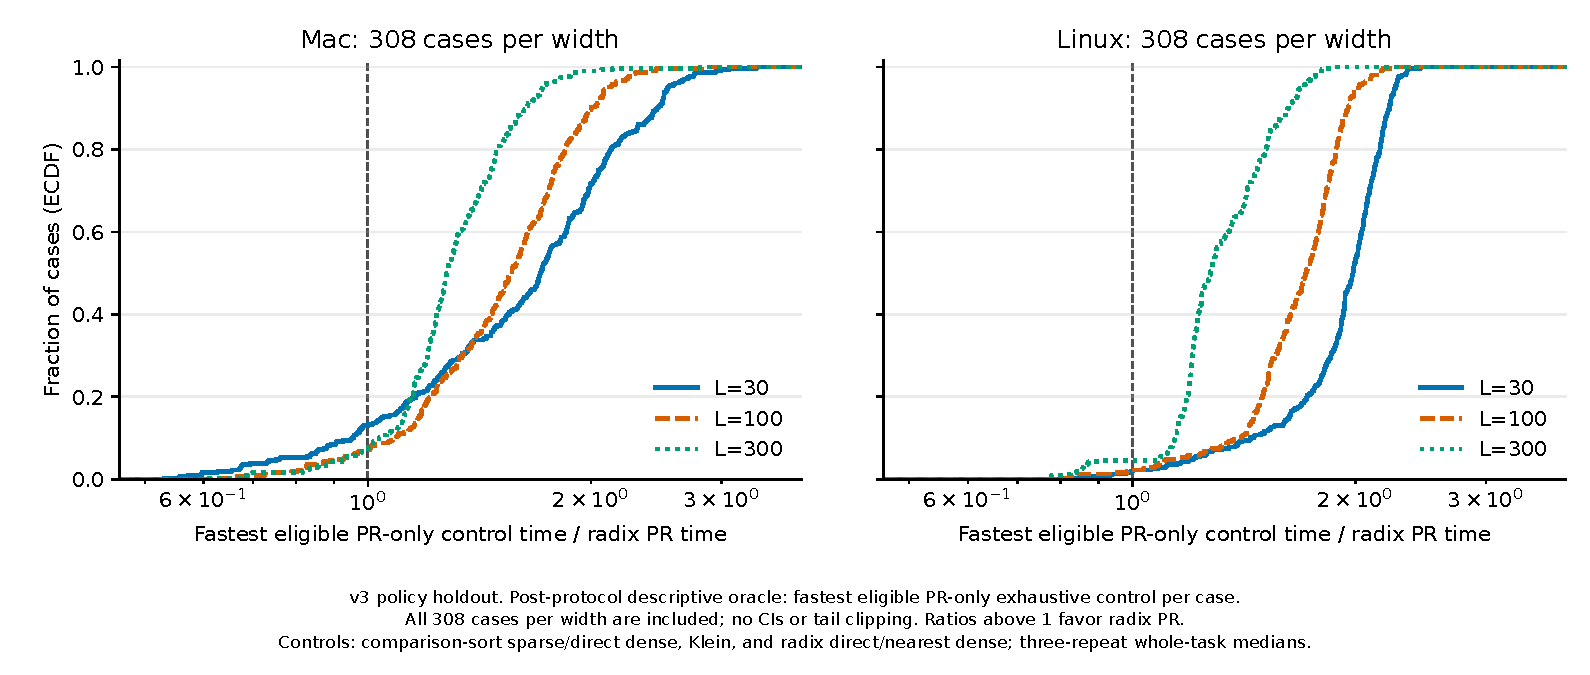
\includegraphics[width=\linewidth]{figures/pr-only-oracle-ecdf.pdf}
\caption{Post-protocol oracle ECDFs for the v3 policy holdout: all 308 cases at each width on each platform, without tail clipping. The horizontal coordinate is the fastest eligible exhaustive PR-only control's whole-task case median divided by exact sparse-radix PR time. Values above one favor radix PR. The five eligible controls are specified in the text; no oracle confidence intervals are computed.}
\label{fig:radix-oracle}
\end{figure*}

\paragraph{Separate racing decisions and scope.}
The frozen comparison-order racing decision at $L=30$ is Mac \textbf{FAIL}, Linux \textbf{FAIL}; the separate radix-order racing decision is Mac \textbf{FAIL}, Linux \textbf{FAIL}.
The first requires both interval lower bounds above one against comparison-based sparse PR, direct dense PR, and exact radix PR;
the second additionally requires this against both matched dense radix PR controls.
These decisions include preparation, adaptive queries, and exact completion in each measured task.
Racing outcomes are separate from the exact-radix decision, and failed criteria remain reported.
The v2 development runs remain historical development evidence and are not pooled with this holdout.
Platforms are summarized separately: no cross-run timing pooling is performed.
The Mac was not isolated: its starting snapshot shows an unrelated Python worker near 100 percent CPU, alongside normal desktop activity. Snapshots are not a continuous load trace. Agent test, build, and report execution stopped during timing; lightweight status reads, completed remote-artifact transfers, and document edits continued. No unrelated process was stopped by the experiment.
The Linux confirmation used a separate serial GitHub Actions job; hosted hardware and host background load were outside our control.
This policy holdout uses previously studied corpus families; it is not an external-domain dataset.
The results address the stated workload and tested implementations, without establishing universal superiority.

\par\noindent{\footnotesize Reproducibility receipt (SHA-256 prefixes): Mac report \texttt{c72f2df666c4}, audit \texttt{a9d44deb51fa}; Linux report \texttt{46c6fba361e4}, audit \texttt{577dab610dd4}. The accompanying JSON receipt records full report, measured-source, and generator hashes.}

\paragraph{Absolute workload costs.}
For the 308 primary three-score tasks, sums of per-task median times are
Mac: 3.094, 10.204, and 60.186 seconds (sparse radix, matched nearest dense radix, and fast-VUS, respectively).
Linux: 2.318, 11.610, and 26.032 seconds (sparse radix, matched nearest dense radix, and fast-VUS, respectively).
At $L=300$, the corresponding sums are Mac: 10.229, 80.733, and 479.670 seconds.
Linux: 11.249, 100.601, and 221.037 seconds.
These quantify operator cost across a stored-score collection; they are
sums of separately timed medians, not measured batch wall times. They exclude
score generation and I/O and do not establish a detector-pipeline speedup.

\subsection{Directly timed stored-score collection workflow}
\label{sec:collection-workflow}
A separate protocol measures an actual local collection operation, beyond
sums of separately timed task medians. Each pass reopens 308 uncompressed
NPZ files, materializes the labels and three original score arrays, makes
924 full PR calls at $L=30$, selects all best-model ties per series, and
serializes the values and decisions into one JSON file. Inputs are the same
17-family policy holdout; no detector inference occurs in this operation.
The stored files total 379,354,532 bytes. Each method uses the unchanged
released implementation and exhaustive thresholds. All validation and
preparation inside the public calls are timed.

The whole monotonic clock runs from before the first NPZ open until the
result file is closed. Imports and synthetic dtype-matched JIT warmup occur
once before timing; input hashing and explicit filesystem-cache warming
precede every pass. Every measured
pass rereads and decodes the files; it is a warm-filesystem workflow, not a
cold-disk or durable-write benchmark (no \texttt{fsync}). Three replications
run serially with one numerical thread on the M1 Pro. Seeded method order
was frozen before timing; its draw places dense last in all three
replications, so order is randomized but not position-balanced. The active
desktop was not isolated; background OCR/Python activity was recorded before
execution. Agent tests, builds and other benchmarks were stopped.

\begin{table*}[t]
\centering\small
\caption{Measured collection wall times in seconds. The last two columns
are separately summarized phase medians, not additive whole-time estimates.
All nine passes and all numeric outputs are retained.}
\label{tab:collection-workflow}
\begin{tabular}{lrrrrrr}
\toprule
Method & Run 1 & Run 2 & Run 3 & Whole median & Metric median & Read median\\
\midrule
Sparse radix PR & 2.902 & 3.187 & 3.721 & 3.187 & 2.816 & 0.299 \\
Dense nearest radix PR & 11.456 & 10.944 & 11.298 & 11.298 & 10.605 & 0.413 \\
Klein fast-VUS PR & 59.041 & 63.647 & 63.749 & 63.647 & 62.493 & 0.927 \\
\bottomrule
\end{tabular}
\end{table*}
Every selected-model set agrees across all nine passes for all 308 series.
The maximum pairwise PR difference is $1.332\times10^{-15}$, below the frozen
$10^{-11}$ tolerance; model ties use $10^{-10}$. Sparse radix takes 3.187 seconds at the median,
giving descriptive whole-workflow ratios of $3.545\times$
against matched dense radix and $19.973\times$ against Klein.
Both comparisons satisfy the frozen median-time criterion. Three observations
per method do not establish a confidence interval or timing significance.
This directly demonstrates savings for the specified stored-score operation;
it does not measure a full training/inference pipeline, production deployment,
or a new-domain evaluation. An independent standard-library auditor
checks recorded order, counts and clock consistency and recomputes
numeric comparisons and decisions from public hash-bound receipts,
without raw input arrays or a new timing measurement.


\subsection{Incremental saturation: primary failure and larger-width gains}
All 666 cases across Mac development, Mac external and Linux external meet
the frozen $10^{-11}$ PR tolerance. Maximum absolute discrepancy is
$1.34\times10^{-15}$ on development and $3.67\times10^{-15}$ on each
external run, rounded upward. An independently written dense oracle also
constructs ramps, components, complete global thresholds and both integrals
without production geometry/integration helpers. Its 8,606 small exhaustive
and adversarial cases include tied scores, widths through $2n+1$ and
noncontiguous inputs. Across 51,636 public calls, maximum discrepancies are
$3.34\times10^{-16}$ for paired output and $2.23\times10^{-16}$ for PR-only,
rounded upward. These checks concern the frozen position-prefix code;
they do not certify new complete-tie code or arbitrary floating-point inputs.

\textbf{The incremental primary runtime criterion fails in all three runs.}
At $L=30$, median ratios against released sparse radix are 1.016, 1.026 and
1.013, with 52/126, 19/48 and 21/48 candidate losses. The criterion does not
hold against every matched control. Table~\ref{tab:saturation-all-controls}
retains all eight controls, widths and slower-case counts. Large ratios
against external libraries include the support-event and ranking improvements
already present in the basic evaluator; they do not establish the marginal
benefit of saturation.
% Generated by experiments/render_saturation_paper_results.py; do not edit data by hand.
% Evidence SHA256: aa3eb2bfd095ba0f54cde12721f0254e04cdd2a7456ab2cb593e0ce8270a8b34
% Renderer SHA256: 189c745a0754b9b568b5a896991a351828668d57ab4b6238256e55103a520c14
% Independent auditor SHA256: 261303ab275b6afce8cfb1160955fd5f6bd88bfdd17b950e190eec39861ba4ab
\begin{table*}[t]
\centering
\footnotesize
\setlength{\tabcolsep}{2.5pt}
\renewcommand{\arraystretch}{1.10}
\begin{tabular}{l*{9}{r}}
\toprule
 & \multicolumn{3}{c}{Mac development} & \multicolumn{3}{c}{Mac external} & \multicolumn{3}{c}{Linux external} \\
\cmidrule(lr){2-4}\cmidrule(lr){5-7}\cmidrule(lr){8-10}
Control & $L=30$ & $L=100$ & $L=300$ & $L=30$ & $L=100$ & $L=300$ & $L=30$ & $L=100$ & $L=300$ \\
\midrule
Full active scan & 1.005(59) & 1.057(38) & 1.271(15) & 1.007(22) & 1.041(14) & 1.216(3) & 1.017(19) & 1.063(9) & 1.218(2) \\
Last-positive stop & 1.011(54) & 1.040(42) & 1.198(21) & 1.012(22) & 1.059(13) & 1.136(6) & 1.025(19) & 1.041(12) & 1.152(6) \\
Released radix & 1.016(52) & 1.191(14) & 1.660(1) & 1.026(19) & 1.151(2) & 1.506(0) & 1.013(21) & 1.202(3) & 1.627(0) \\
Dense nearest radix & 2.602(5) & 4.607(0) & 8.107(0) & 2.835(0) & 6.250(0) & 13.188(0) & 3.274(0) & 7.689(0) & 13.526(0) \\
fast-VUS & 20.175(0) & 41.291(0) & 72.435(0) & 16.908(0) & 42.627(0) & 92.597(0) & 13.174(0) & 28.616(0) & 57.738(0) \\
Sparse comparison sort & 2.041(9) & 2.087(6) & 2.285(0) & 1.783(5) & 1.816(5) & 1.997(4) & 1.630(9) & 1.678(8) & 1.993(8) \\
Dense direct & 3.286(3) & 5.518(0) & 10.557(0) & 3.478(0) & 6.401(0) & 13.643(0) & 3.657(0) & 8.412(0) & 14.453(0) \\
Dense direct radix & 2.672(5) & 4.970(0) & 10.124(0) & 3.008(0) & 6.218(0) & 13.439(0) & 3.023(0) & 7.705(0) & 14.128(0) \\
\midrule
Fastest eight-control oracle & 0.978(84) & 1.006(60) & 1.136(24) & 0.980(32) & 1.023(19) & 1.113(9) & 0.984(29) & 1.030(18) & 1.142(10) \\
\bottomrule
\end{tabular}
\caption{Median paired runtime ratio (control divided by saturation), with the number of slower saturation cases in parentheses. Cases per width: Mac development: 126; Mac external: 48; Linux external: 48. A ratio below one favors the control. Each case uses the median of three complete public-call timings. The oracle selects the fastest of the eight measured controls separately for each case, after measurement. All cases and widths are retained. Frozen primary $L=30$ criterion: Mac development: FAIL; Mac external: FAIL; Linux external: FAIL.}
\label{tab:saturation-all-controls}
\end{table*}


At the prespecified stress width $L=300$, ratios against released radix are
1.660 on development, 1.506 on Mac external and 1.627 on Linux external.
There are 125/126, 48/48 and 48/48 candidate wins. External geometric-ratio
bootstrap intervals are [1.417, 2.634] and [1.527, 2.982]; aggregate-ratio
intervals are [1.392, 2.472] and [1.554, 2.993]. Against the retrospective
fastest of all eight controls, median ratios are only 1.136, 1.113 and 1.142,
with 24/126, 9/48 and 10/48 losses. The oracle is not a deployable selector.

At width 300, aggregate saturation visits are 72.1\%, 57.5\% and 57.5\%
of full-active visits; against last-positive visits they are 73.8\%, 58.3\%
and 58.3\%. Median runtime ratios against last-positive stopping are 1.198,
1.136 and 1.152. Reduced traversal does not eliminate preparation, pointer
access or component bookkeeping, and some lower-work cases remain slower.
Seven development series and four external series have one original interval;
interval count alone does not establish the distinct-support-score hypothesis.

A separate 16-case structural study crosses four input families with
$L\in\{32,128,512,2048\}$ and $n=4L+3$. All cases meet the frozen count
predictions and agree with released radix within $1.39\times10^{-17}$.
The distinct singleton visits $3L-1$ positions, and the two-original
separating family visits $4L$; the all-tied singleton visits all active
support. These are constructed mechanism checks, not estimates of
real-data prevalence or a numerical comparison to another dense oracle.
The complete per-case timings and the all-tied negative control remain
in the structural-study artifact.

\subsection{Paired external supplement and cross-platform scope}
A separately frozen descriptive supplement compares paired ROC--PR public
calls at $L=30$ on the 48 external score vectors, with three warmed complete
repetitions. Actual pinned Benchopt completes all 48 cases, with median
ratio $34.918\times$ and minimum $20.079\times$. Released paired radix has
median ratio $1.017\times$ with 19/48 candidate losses. This is a separate
workload from the whole-evaluator three-score tasks and is not pooled with
the Benchopt ratios in Table~\ref{tab:radix-primary}.

DTAI~\cite{dtaianomaly} is prescribed for the Isolation Forest vector of each of the 12 series.
Ten complete all repetitions; PSM and swan hit the 30-second parent watchdog
on their first timed call and later repetitions are skipped. The completed
subset's median ratio is $101.106\times$; the two censored cases have no
fabricated duration or ratio. Native parallel/fast-math compilation is
retained, with one compute thread. Completed paired outputs agree within
$8.22\times10^{-15}$. This supplement changes neither primary decision.

The external Linux workflow regenerates the specified inputs from pinned
sources. Raw data and labels match Mac hashes; 11/48 score arrays match
byte for byte and 37 differ after platform-dependent score generation.
All 53 downloaded artifact-file hashes were checked. This reproduces the
input-generation procedure and evaluator experiment, not an identical-array
replay or an independent laboratory study.

\subsection{Run aggregation: structured ties and a fragmentation control}
The separately frozen run study evaluates 20 constructed cases (five score
families at $L=32,128,512,2048$) and every one-interval case from the previous
development and external corpora: 63 and 48 cases, respectively. This is
reused-data evaluation, not unseen confirmation. All four methods are PR-only
and include validation, ranking, geometry and, for run aggregation, the
square-root table. Each case has one untimed warm call per method and five
seeded randomized serial repetitions on the Apple M1 Pro with one compute
thread (Python 3.12.4, NumPy 1.26.4, Numba 0.59.1).

All 131 cases satisfy the numerical and work assertions. The maximum absolute
discrepancy from released radix is $5.56\times10^{-16}$. Every width visits at
most $3P_0$ score classes. For the all-tied singleton at $L=2048$, run aggregation
inspects 2,049 runs in total, while the position scan visits 2,099,201 positions.
These counts support the proved separation; they do not determine wall time.

A separate untimed verifier compares 650 random cases against direct dense
evaluation (maximum absolute difference $3.34\times10^{-16}$), and 36 small
complete integrals against independently constructed Decimal arithmetic at
80-digit precision (maximum $2.60\times10^{-16}$). It also checks every one of
150,000 integer prefixes against Python integers, 20,009 synthetic limb
subtractions, and 6,569 per-width counter reconstructions. These are internal
implementation checks, separate from benchmark cases and the local error theorem.

Table~\ref{tab:tie-structural} reports every constructed family at the largest
width. Larger ratios favor run aggregation; subunit ratios are regressions.
The alternating-score control defeats compression because each score class is
highly fragmented. Distinct scores also offer little aggregation benefit.
These are constructed witnesses, not a sample of operational detectors.

\begin{table}[t]
\centering\small
\caption{Constructed $L=2048$ cases, $n=8195$: comparator / run-aggregation median
time. All five families retained; full results at every width are in the artifact.}
\label{tab:tie-structural}
\begin{tabular}{lrrr}
\toprule
Scores / labels & Active prefix & Radix & Fast-VUS\\
\midrule
All tied / singleton & 8.816 & 29.386 & 739.615 \\
Distinct / original last & 0.947 & 32.919 & 765.564 \\
Eight blocks / singleton & 5.126 & 31.187 & 789.399 \\
Alternating / singleton & 0.277 & 1.216 & 41.319 \\
All tied / interval of 8 & 8.867 & 29.487 & 739.147 \\
\bottomrule
\end{tabular}
\end{table}

The real-score results in Table~\ref{tab:tie-real} are deliberately separate.
At $L=300$, run aggregation loses to active prefix on 16 of 21 development
cases and 14 of 16 external cases. It is therefore an option for compressible
ties, not a replacement justified by broad real-data gains. No runtime selector
or population confidence interval is inferred from these reused cases.

\begin{table}[t]
\centering\small
\caption{All reused one-interval cases. Each entry is median comparator/run
ratio, followed by the number of run-aggregation losses.}
\label{tab:tie-real}
\setlength{\tabcolsep}{4pt}
\begin{tabular}{llrrr}
\toprule
Corpus & $L$ & Active prefix & Radix & Fast-VUS\\
\midrule
Dev. ($n_c=21$) & 30 & 1.010 (10) & 0.984 (14) & 23.606 (0) \\
Dev. ($n_c=21$) & 100 & 0.921 (15) & 0.998 (11) & 49.776 (0) \\
Dev. ($n_c=21$) & 300 & 0.857 (16) & 1.156 (9) & 58.776 (0) \\
Ext. ($n_c=16$) & 30 & 1.014 (5) & 1.007 (5) & 22.197 (0) \\
Ext. ($n_c=16$) & 100 & 0.996 (9) & 1.006 (6) & 51.389 (0) \\
Ext. ($n_c=16$) & 300 & 0.835 (14) & 1.075 (0) & 99.247 (0) \\
\bottomrule
\end{tabular}
\end{table}

The protocol, source inventory, input hashes, five raw repetitions and work
profiles are frozen together. The complete 131-case report includes every
ratio and loss. This study changes neither the whole-method primary PASS nor
the active-prefix primary FAIL decisions.


\section{Limitations and reproducibility}
The computational target is a pinned scalar metric, not every historical
VUS variant or the complete threshold surface. Exact evaluation does not
establish that this metric is the best scientific measure of anomaly
quality. Support-event gains depend on sparse expanded support. Position
prefixes may remain long because of component coverage or large ties;
complete-tie aggregation requires one original interval and charges score-class
fragmentation. At fixed small $L$, the preceding radix evaluator is already
linear in $n$, so an asymptotic growing-width separation does not itself
promise a default-width speedup.

The proof model fixes score keys to binary64 and treats metric arithmetic,
including square roots, as unit cost. It is not an arbitrary-precision
bit-complexity analysis. Integer-prefix accumulation exactly sums rounded
roots and the integer test certifies a sufficient stopping condition; the
local mass guarantee does not establish correct rounding of the final scalar.
Measured equality is tolerance-based. No general all-input floating-point
error certificate or universal CPU/GPU ranking is claimed.

The external corpus is small and its four score generators share CPU
preprocessing. Hardware findings are limited to recorded environments,
including workstation background activity and hosted-runner variability.
The earlier whole-evaluator corpus has previously studied source families.
All losses, censored cases, failed incremental criteria and negative optional
racing outcomes are retained. Optional width refinement and racing are not
contributions of this paper; their derivations and failed runtime decisions
remain in the versioned supplementary artifact~\cite{sparsevus03}.

The public repository contains source, tests, proofs, independent oracles,
source/input hashes, frozen protocols, raw measurements and reconstruction
scripts. Frozen historical evaluators are preserved alongside new candidate
code. Data are fetched from pinned public sources; raw third-party data are
not relicensed or bundled, and source-specific terms are documented.

\paragraph{AI assistance disclosure.}
OpenAI Codex assisted with literature retrieval, algorithm and proof
development, implementation, experiment orchestration, testing and manuscript
drafting. Separately prompted agent contexts constructed oracles and reviewed
claims within the same workflow. These checks are internal verification,
not independent laboratory replication or external peer review. The artifact
records code and measured evidence; AI tools are not listed as authors.

\section{Conclusion}
Sparse VUS evaluates the exhaustive dynamic scalar metric through support
events with exact contributions for omitted thresholds. Fixed-key ranking
and interval geometry give a support-sensitive baseline; width activation
and component unions make further work depend on a saturated prefix.
For one original interval, temporal runs aggregate complete tied classes,
with an integer sufficient stopping condition and a separate local numerical
bound. Whole-evaluator acceleration and incremental prefix acceleration are
different empirical claims: the first passes its stated primary study,
while the latter fails its default-width criterion and improves qualified
larger-width regimes.

\bibliographystyle{ACM-Reference-Format}
\bibliography{sparse_vus_references}
\end{document}
